% @author Marcel Ruland (2018)

%\cite{han12}
%\cite{rohlfing18}


\chapter{Method}
\section{Association Rules}
In the following, I will first lay out the type of association rule used by \citeasnoun{rohlfing18} and then explain how I modified this scheme to better fit the linguistic, interactional nature of the data. The basic sequence is structured as follows:
\begin{quote}
	\code{<(A [1,3]),(A,B [3,4]),(A,B,C [4,7]),(C [7,9])(A,B,C [9,13])>}
\end{quote}

\begin{figure}
	\center
	% @author Marcel Ruland (2018)
{\sffamily\addfontfeature{Numbers=Lining,Letters=Uppercase}
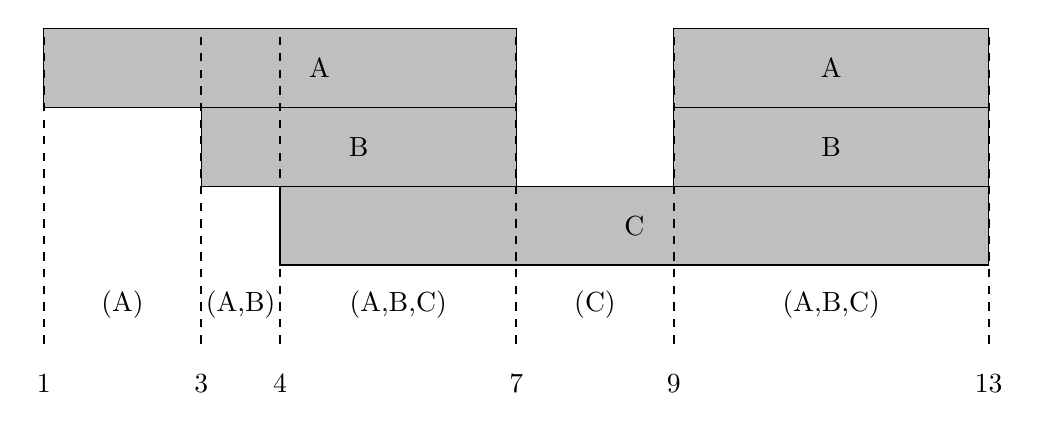
\begin{tikzpicture}
%	\draw [help lines, dashed] (0,0) grid (12,5);  % help lines
	
	% boxes
	\draw [fill=lightgray] (0,4) rectangle (6,5);  % A1
	\node at (3.5,4.5) {A};
	
	\draw [fill=lightgray] (8,4) rectangle (12,5);  % A2
	\node at (10,4.5) {A};
	
	\draw [fill=lightgray] (2,3) rectangle (6,4);  % B1
	\node at (4,3.5) {B};
	
	\draw [fill=lightgray] (8,3) rectangle (12,4);  % B2
	\node at (10,3.5) {B};
	
	\draw [fill=lightgray] (3,2) rectangle (12,3);  % C
	\node at (7.5,2.5) {C};
	
	% item sets
	\node at (1,1.5) {(A)};
	\node at (2.5,1.5) {(A,B)};
	\node at (4.5,1.5) {(A,B,C)};
	\node at (7,1.5) {(C)};
	\node at (10,1.5) {(A,B,C)};
	
	% time points
	\node at (0,0.5) {1};
	\node at (2,0.5) {3};
	\node at (3,0.5) {4};
	\node at (6,0.5) {7};
	\node at (8,0.5) {9};
	\node at (12,0.5) {13};
	
	% time point lines
	\draw [dashed, thick] (0,1) -- (0,5);
	\draw [dashed, thick] (2,1) -- (2,5);
	\draw [dashed, thick] (3,1) -- (3,5);
	\draw [dashed, thick] (6,1) -- (6,5);
	\draw [dashed, thick] (8,1) -- (8,5);
	\draw [dashed, thick] (12,1) -- (12,5);
	
	% text representation
%	\node at (6,0) {\code{<(A [1,3]),(A,B [3,4]),(A,B,C [4,7]),(C [7,9])(A,B,C [9,13])>}};
\end{tikzpicture}
}
	\caption{Graphical representation of a sequence}
	\label{fig:sequence}
\end{figure}

In traditional sequential pattern mining, the basic data type---called a sequence---is an ordered set of (unordered) item sets. Here, every item set in the sequence has an additional annotation marking the start and end time points between which the item set is contained in the data.
%zero delay only in intrapersonal rules, minimum delay for interpersonal rules -- reaction time